% !TeX root=../main.tex

\section{Preliminaries}
\label{sec:models}
We introduce the basic notions of the formal transition systems and trace alignments that will be used henceforth.

\subsection{Transition Graphs}\label{subsec:ppn}

We consider an abstract model for representing the traces from a process which is based on graphs. These
graphs, which we call \emph{transition graphs} and formalise below, can be further equiped with edge-labels expressing 
the probability of a transition, and hence of a specific trace. The following definition is based on \cite{GartnerFW03}.
\todo{note!! changed the definition of $L$}

\begin{definition} A \emph{(probabilistic) transition graph} (TG) is a tuple $(V,s,t,L,R)$ where:
  \begin{inparaenum}[\itshape (i)]
    \item $V \subset \mathbb{N}$ is a set of \emph{nodes};
    \item $s\in V$ is the \emph{initial node};
    \item $e\in V$ is the \emph{accepting node};
    \item $L: V \to \alphabet$ is the \emph{node labelling function};
    \item $R: V \times V \rightarrow [0,1]$ is a \emph{(probabilistic) transition matrix} indicating, for each pair of nodes, 
    	what is the probability that executing a transition from the first node leads to the second node.
  \end{inparaenum}
Thus $R$ is such that for  every $\ind{i} \in V$, $\sum_{\ind{j}\in V}[R]_{\ind{ij}}=1$.
%
A \emph{weigthed (probabilistic) transition graph} is a pair $(G,\omega)$ where $G$ is a (probabilistic) TG and 
$\omega\in[0,1]$ is its \emph{weight}.
\end{definition}
%
The condition for $R$ ensures that its values can be interpreted as a probability distribution for choosing the next node upon 
executing a transition. $L$ and $R$ determine the probability of reaching a node labeled by $\beta\in\Sigma$ from any node 
labeled $\alpha\in\Sigma$ in $n$ steps by 
$[G.\Lambda^n]_{\alpha\beta}:=L^{-1}(a)R^n L^{-1\top}b$, 
where $L^{-1}$ is seen as a vector (see Example \ref{ex:wheredotiszero}).

\begin{figure}[!t]
	\begin{minipage}{.49\textwidth}\centering 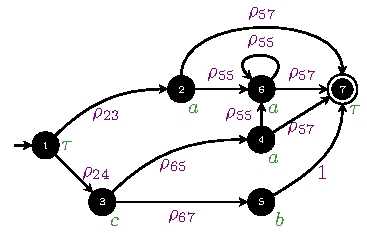
\includegraphics[width=.8\textwidth]{images/closed_example.pdf}
	\caption{A probabilistic TG with abstract weights.}\label{fig:lmc}
\end{minipage}
\end{figure}
%
\figurename~\ref{fig:lmc} shows a TG with the obvious interpretation; an edge from node $\ind{i}$ to node $\ind{j}$ is shown 
(with its weight) only if the transition probability $[\tg.R]_{\ind{i}\ind{j}}$ is positive.
%
A \emph{valid sequence} of the TG $\tg$ is a path $\ind{i}_0\ldots\ind{i}_n$ of nodes in $\tg.V$ from the initial to the 
accepting node using only transitions with positive probability:
\begin{inparaenum}[\it (i)]
\item $\ind{i}_0 = \tg.s$;
\item $\ind{i}_n = \tg.e$;
\item for every $j \in \set{1,\ldots,n}$ we have $[R]_{\ind{i}_{j-1}\ind{i}_{j}} > 0$.
\end{inparaenum}
Runs and model traces of TGs are defined in the obvious manner. We use the same notation to indicate the runs underlying a 
model trace, and the valid sequences underlying a run. The computation of probabilities for runs and traces is defined equivalently.

\subsection{Kernels and Trace Kernels}\label{subsec:katk}
As a foundational basis to compute trace alignments, we adapt similarity measures from the database literature.  Given a set 
of data examples $\mathcal{X}$, a (positive definite) \emph{kernel} function 
$k\colon \mathcal{X}\times \mathcal{X}\to \mathbb{R}$ denotes the similarity of elements in $\mathcal{X}$. If $\mathcal{X}$ is 
the $d$-dimensional Euclidean Space $\mathbb{R}^d$, the simplest kernel function is the inner product 
$\Braket{\mathbf{x},\mathbf{x}'}=\sum_{1\leq i\leq d}\mathbf{x}_i\mathbf{x}'_i$.
A kernel \emph{performs ideally} if $k(x,x')=1$ whenever $x$ and $x'$ are the same object (\textit{strong equality}) and 
$k(x,x')=0$ whenever $x$ and $x'$ are distinct objects (\textit{strong dissimilarity}). It is \emph{appropriate} when similar 
elements $x,x'\in\mathcal{X}$ are close in the feature space. Note that appropriateness can be only assessed 
empirically \cite{Gartner03}.
A positive definite kernel induces the distance metric
\begin{equation}\label{eq:dofk}
d_k(\mathbf{x},\mathbf{x}'):=\sqrt{k(\mathbf{x},\mathbf{x})-2k(\mathbf{x},\mathbf{x}')+k(\mathbf{x}',\mathbf{x}')}
\end{equation}
If the kernel is the inner product, this defines the Euclidean distance $\norm{\mathbf{x}-\mathbf{x}'}{2}$. A normalized vector 
$\hat{\mathbf{x}}$ is defined as $\mathbf{x}/\norm{\mathbf{x}}{2}$. In this case, 
$\norm{\hat{\mathbf{x}}-\hat{\mathbf{x}}'}{2}^2=2(1-\Braket{\hat{\mathbf{x}},\hat{\mathbf{x}}'})$ holds.
%
If $\mathcal{X}$ does not represent a $d$-dimensional Euclidean space, we can use an \emph{embedding} 
$\embed\colon\mathcal{X}\to \mathbb{R}^d$ to define a kernel $k_\embed\colon \mathcal{X}\times \mathcal{X}\to\mathbb{R}$ 
as $k_\embed(x,x'):=\Braket{\embed(x),\embed(x')}$. As a result, $k_\embed(x,x')=k_\embed(x',x)$ for each 
$x,x'\in\mathcal{X}$.

The literature provides a kernel representation for strings \cite{LodhiSSCW02,GartnerFW03}, which we employ for 
traces. We provide an intuition for the desired features of this representation. If we associate each dimension in $\mathbb{R}^d$ 
to a different subtrace $\alpha\beta$ of size $2$ (i.e., $2$-grams%
\footnote{In fact, $p$-grams of arbitrary length $p\geq 2$ might be adopted \cite{Gartner03}. Larger $p$s improve precision 
but increase the computational complexity of considering all subtraces of length $p$ whose elements occur at any 
distance from each other within the trace.}), 
the associated coordinate should represent the frequency and ``compactness'' of this subtrace within the trace $\trace$ of 
interest. Therefore, we introduce a \emph{decay factor} $\lambda\in[0,1]\subseteq\mathbb{R}$ that, for all $m$ subtraces where $\alpha$ and $\beta$ appear in $\trace$ at the same relative distance $\delta < |\trace|$, weights the resulting embedding as $\lambda^\delta m$.
%
We lift this approach to consider all occurrences of subtraces $\alpha\beta$ at every distance between $1$ and $|\trace|-1$
in two steps. First, we encode $\trace$ into a ``linear'' TG $\tg_\trace$ (\figurename~\ref{fig:taustar}) in the obvious way. 
%
\begin{figure}[!t]
	\centering
	\includegraphics[width=.35\textwidth]{images/taustar.pdf}
	\caption{Graphical representation of the TG encoding trace $\const{caba}$.}
	\label{fig:taustar}
\end{figure}
%
Then, we compute a simplified version of the embedding from \cite{LodhiSSCW02} as 
$\trembed_{\alpha\beta}(\trace)=\sum_{1\leq i\leq |\trace|}\lambda^i[(\tg_{\trace}.\Lambda)^i]_{\alpha\beta}$. 
The kernel between two traces corresponds to the sum of the products of such values calculated 2-gram by 2-gram for the two 
traces. This trace kernel returns strong dissimilarity when the two traces have no shared 2-grams at any arbitrary occurring length, 
but does not enjoy strong equality: the similarity of a trace with itself is at least $\lambda^2$ - returned when the trace is a 
2-gram.

%
%we can represent it as a TG \cite{Myers1989} $(1,{|\tau|},L_\tau,R_\tau,1)$ having $[L_\tau]_{{\color{green}\alpha}\texttt{\color{blue}i}}=1\Leftrightarrow \tau_{\texttt{\color{blue}i}}={\color{green}\alpha}$ and $[L_\tau]_{{\color{green}\alpha}\texttt{\color{blue}i}}=0$ otherwise, and $\forall i<|\tau|.\; [R_\tau]_{\texttt{\color{blue}i(i+1)}}=1 $ and $[R_\tau]_{\texttt{\color{blue}ij}}=0$ otherwise.
%Exploiting this encoding, we can adopt a simplified version of the embedding defined in \cite{LodhiSSCW02,Raedt} as $\embed_{\mathcal{T}}(\tau)_{{\color{green}\alpha\beta}}=\sum_{1\leq i\leq |\tau|}\lambda^i[(\Lambda_\tau)^i]_{\color{green}\alpha\beta}$.
%Please note that this definition is similar to a transition matrix embedding proposed in \cite{GartnerFW03} via geometric series, that is $\sum_i\lambda^i[R^i]_{\color{green}\alpha\beta}$.

%\begin{example}\label{ex:tracembed}
%	{Let us suppose that we want to align a trace $\tau^*$ to one of the traces from a transition graph: in order to carry out an approximate alignment, we need to transform it to a transition graph first.} A trace $\tau^*=\textup{caba}$ can be graphically represented in Figure \ref{fig:taustar}. The associated TG $T=(\mathtt{\color{blue}1},\mathtt{\color{blue}4},L,R,1)$ has matrices $L$ and $R$  defined as follows:
%	$$L:=\kbordermatrix{
%		& \texttt{\color{blue}1}&\texttt{\color{blue}2}&\texttt{\color{blue}3}&\texttt{\color{blue}4}\\
%		\color{green}a            & 0&\textbf{1}&0&\textbf{1}\\
%		\color{green}b            & 0&0&\textbf{1}&0\\
%		\color{green}c            & \textbf{1}&0&0&0\\
%	}\qquad R:=\kbordermatrix{
%		& \texttt{\color{blue}1}&\texttt{\color{blue}2}&\texttt{\color{blue}3}&\texttt{\color{blue}4}\\
%		\texttt{\color{blue}1}  & 0&\color{red}1&0&0\\
%		\texttt{\color{blue}2}  & 0&0&\color{red}1&0\\
%		\texttt{\color{blue}3}  & 0&0&0&\color{red}1\\
%		\texttt{\color{blue}4}  & 0& 0& 0& 0\\
%	}$$
%We can similarly represent all the traces from the USPN.
%\end{example}

%\begin{example}
%The subtrace \textit{\textbf{\uline{hi}}} is represented in \textit{\textbf{\uline{hi}}deous},   \textit{\uline{\textbf{h}}e\uline{{i}}d\textbf{i}}, and \textit{\uline{{\textbf{h}i}}nd\textbf{i}}, but with different frequencies and subtrace distances. We have $\embed_{\mathcal{T}}(\textit{hideous})_{{\color{green}hi}}=\lambda$,  $\embed_{\mathcal{T}}(\textit{heidi})_{{\color{green}hi}}=\lambda^2+\lambda^4$, and $\embed_{\mathcal{T}}(\textit{hindi})_{{\color{green}hi}}=\lambda+\lambda^4$.
%\end{example}



\begin{table}[t!]
\vspace{+0.5cm}
\caption{Embedding of traces $\const{caba}$, $\const{caa}$ and $\const{cb}$.}\label{tb:embedding}
%\vspace{-0.3cm}
\centering
\resizebox{0.9\columnwidth}{!}{
	\begin{tabularx}{1.1\columnwidth}{
>{\hsize=.15\hsize}X
>{\hsize=.15\hsize}X
>{\hsize=.1\hsize}X
>{\hsize=.1\hsize}X
>{\hsize=.1\hsize}X
>{\hsize=.1\hsize}X
>{\hsize=.1\hsize}X
>{\hsize=.25\hsize}X
>{\hsize=.15\hsize}X
>{\hsize=.1\hsize}X
}
		\toprule
		& $\const{aa}$    & $\const{ab}$   & $\const{ac}$    & $\const{ba}$   & $\const{bb}$   & $\const{bc}$ & $\const{ca}$ & $\const{cb}$ & $\const{cc}$   \\
		\midrule
		$\const{caba}$ & $\lambda^2$ & $\lambda$ & $0$ & $\lambda$  & $0$  & $0$ & $\lambda+\lambda^3$ & $\lambda^2$ & $0$\\
		%$\const{caaa}$ & $2\lambda+\lambda^2$& $0$ & $0$ & $0$ & $0$ & $0$ & $\lambda+\lambda^2+\lambda^3$ & $0$ & $0$ \\
		$\const{caa}$  & $\lambda$ & $0$ & $0$ & $0$ & $0$ & $0$ & $\lambda+\lambda^2$ & $0$&  $0$\\
		$\const{cb}$   & $0$ & $0$ & $0$ & $0$ & $0$ & $0$ & $0$ & $\lambda$& $0$ \\
		\bottomrule
	\end{tabularx}
}
\vspace{-0.5cm}
\end{table}

\begin{example}\label{ex:wheredotiszero} %\small
The possible 2-grams over $\tasks=\Set{a,b,c}$ are 
$\tasks^2=\Set{\const{aa},\const{ab},\const{ac},\const{ba},\const{bb},\const{bc},\const{ca},\const{cb},\const{cc}}$. 
Table~\ref{tb:embedding} shows the embeddings of some traces. The 2-gram $\const{cb}$ has only one nonzero component 
(itself) with $\trembed_{\const{cb}}(\const{cb})=\lambda$. Trace $\const{caa}$ has the 2-gram $\const{ca}$ occurring with 
length $1$ ($\const{\underline{ca}a}$) and $2$ ($\const{\underline{c}a\underline{a}}$), and the 2-gram $\const{aa}$ with 
length $1$ ($\const{c\underline{aa}}$). Hence: $\trembed_{\const{ca}}(\const{caa})=\lambda+\lambda^2$ and 
$\trembed_{\const{aa}}(\const{caa})=\lambda$. 
We compute the similarity between the trace $\const{caba}$ and the other two traces. To do so, we sum, column by column 
(i.e., 2-gram by 2-gram) the product of the embeddings for each pair of traces. We get 
$k_{\trembed}(\const{caba},\const{caa})=\lambda^3+(\lambda+\lambda^3)(\lambda+\lambda^2)$ and 
$k_{\trembed}(\const{caba},\const{cb})=\lambda^3$,
which induces ranking $
k_{\trembed}(\const{caba},\const{caa})>
k_{\trembed}(\const{caba},\const{cb})
$.
\end{example}



%%%%%%%%%%%%%%%%%%%%%%%%
%%%%%%%%%%%%%%%%%%%%%%%%
%%%% END INPUT
%%%%%%%%%%%%%%%%%%%%%%%%
%%%%%%%%%%%%%%%%%%%%%%%%

\endinput
\subsection{Graph Embedding}\label{ssec:ge}
Graph kernels allow mapping graph data structures to feature spaces (usually an Euclidean space in $\mathbb{R}^n$ for $n\in \mathbb{N}_{>0}$) \cite{Samatova} so to express graph similarity functions that can then be adopted for both classification \cite{TsudaS10} and clustering algorithms. One of the first approaches used in literature involved the definition of topological description vectors \cite{Sidere} for each graph in a graph database, for then defining the graph similarity function as an inner product of their associated vectors. One inconvenience of such a technique is that it is required to perform NP-complete subgraph isomorphisms among a collection of graphs. It has been already proved that the definition of a graph kernel function fully recognizing the structure the graph always boils down to solving such NP-Complete problem \cite{GartnerFW03}, as exact embeddings generable in polynomial can be inferred just for loop-free Direct Acyclic Graphs \cite{BergamiBM20}.


Consequently, most recent literature focused on extracting relevant features of such graphs, that are then used to define a graph similarity function. The most common approach adopted in the kernel to extract such features is called \textit{propositionalization}: we might extract all the possible features (e.g., subsequences), and then define a kernel function based on the occurrence and similarity of these features \cite{Gartner03}.

%\section{LTL over Finite Traces and the Declare Framework}
%\label{sec:preliminaries}
%As a formal basis for specifying crisp (temporal) business constraints, we adopt the customary choice of Linear Temporal Logic over finite traces (\LTLf \cite{DeVa13,DDGM14}). This logic is at the basis of the well-known \declare \cite{PeSV07} constraint-based process modeling language.
%We provide here a gentle introduction to this logic and to the \declare framework.
%
%\subsection{Linear Temporal Logic over Finite Traces}
%
%$\LTLf$ has exactly the same syntax as standard $\LTL$, but, differently from $\LTL$, it interprets formulae over an unbounded, yet finite linear sequence of states. Given an alphabet $\Sigma$ of atomic propositions (in our setting, representing activities), an \LTLf formula $\varphi$ is built by extending propositional logic with temporal operators:
%\[\varphi ::= a \mid \lnot \varphi \mid \varphi_1\lor \varphi_2
% \mid \Next\varphi \mid \varphi_1\Until\varphi_2 \quad \text{ where $a \in \Sigma$.}\]
%
%
%%The semantics of \LTLf is given in terms of \emph{finite traces}
%%denoting finite, \emph{possibly empty}, sequences
%%$\tau=\tau_0,\ldots,\tau_n$ of elements from the alphabet $\Sigma$. The evaluation of a formula is done in a given state (i.e., position) of the trace.
%
%
%The semantics of \LTLf is given in terms of \emph{finite traces} denoting finite, \emph{possibly empty} sequences $\tau=\tup{\tau_0, \ldots, \tau_n}$ of elements of $2^\Sigma$, containing all possible propositional interpretations of the propositional symbols in $\Sigma$. In the context of this paper, consistently with the literature on business process execution traces, we make the simplifying assumption that in each point of the sequence, one and only one element from $\Sigma$ holds. Under this assumption, $\tau$ becomes a total sequence of activity occurrences from $\Sigma$, matching the standard notion of (process) execution trace. We indicate with $\tasks^*$ the set of all traces over $\tasks$. The evaluation of a formula is done in a given state (i.e., position) of the trace, and we use the notation $\tau,i\models \varphi$ to express that $\varphi$ holds in the position $i$ of $\tau$. We also use $\tau \models \varphi$ as a shortcut notation for $\tau,0\models\varphi$. This denotes that $\varphi$ holds over the entire trace $\tau$ starting from the very beginning and, consequently, logically captures the notion of \emph{conformance} of $\tau$ against $\varphi$. We also say that $\varphi$ is \emph{satisfiable} if it admits at least one conforming trace.
%
%%We start by giving an intuitive account of the resulting semantics. In the syntax above, operator $\Next$ denotes the \emph{next state} operator, and $\Next \varphi$ is true if $\varphi$ is true is true now if there exists a next state (i.e., the current state is not at the end of the trace), and in the next state $\varphi$ holds. Operator $\Until$ instead is the \emph{until} operator, and $\varphi_1\Until\varphi_2$ is true if $\varphi_1$ holds now and continues to hold until eventually, in a future state, $\varphi_2$ holds. From the given syntax we can derive the usual boolean operators $\land$ and $\rightarrow$, the two formulae $\true$ and $\false$, as well also additional temporal operators. We consider in particular the following three:
%%\begin{compactitem}[$\bullet$]
%%\item (eventually) $\Diamond \varphi = \true \Until \varphi$ is true if there is a future state where $\varphi$ holds;
%%\item (globally) $\Box \varphi = \neg \Diamond \neg \varphi$ is true if now and in all future sates $\varphi$ holds;
%%\item (weak until) $\varphi_1 \Wntil \varphi_2 = \varphi_1\Until\varphi_2 \lor \Box \varphi_1$ relaxes the until operator by admitting the possibility that $\varphi_2$ never becomes true, in this case by requiring that is true if $\varphi_1$ holds now and in all future states.
%%\end{compactitem}
%% To define the semantics formally, we denote the length of trace $\tau$ as $\length(\tau) =  n+1$.
%
%
%In the syntax above, operator $\Next$ denotes the \emph{next state} operator, and $\Next \varphi$ is true if there exists a next state (i.e., the current state is not at the end of the trace), and in the next state $\varphi$ holds. Operator $\Until$ instead is the \emph{until} operator, and $\varphi_1\Until\varphi_2$ is true if $\varphi_1$ holds now and continues to hold until eventually, in a future state, $\varphi_2$ holds. From these operators, we can derive the usual boolean operators $\land$ and $\rightarrow$, the two formulae $\true$ and $\false$, as well as additional temporal operators. We consider, in particular, the following three:
%\begin{compactitem}[$\bullet$]
%\item (eventually) $\Diamond \varphi = \true \Until \varphi$ is true if there is a future state where $\varphi$ holds;
%\item (globally) $\Box \varphi = \neg \Diamond \neg \varphi$ is true if now and in all future states $\varphi$ holds;
%\item (weak until) $\varphi_1 \Wntil \varphi_2 = \varphi_1\Until\varphi_2 \lor \Box \varphi_1$ relaxes the until operator by admitting the possibility that $\varphi_2$ never becomes true, in this case by requiring that $\varphi_1$ holds now and in all future states.
%\end{compactitem}
%%We write $\tau \models \varphi$ as a shortcut notation for $\tau,0\models \varphi$, and say that formula $\varphi$ is \emph{satisfiable}, if there exists a trace $\tau$ such that $\tau \models \varphi$.
%
%\begin{example}
%The $\LTLf$ formula $\Box(\activity{accept} \rightarrow \Diamond\activity{pay})$ models that, whenever an order is accepted, then it is eventually paid. The structure of the formula follows what is called \emph{response template} in \declare.
%\end{example}
%
%%Every $\LTLf$ formula $\varphi$ can be translated into a corresponding standard finite-state automaton $\aut_\varphi$ that accepts all and only those finite traces that satisfy $\varphi$ \cite{DeVa13,DDGM14}. Although the complexity of reasoning with $\LTLf$ is the same as that of $\LTL$, finite-state automata are much easier to manipulate in comparison with B\"uchi automata, which are necessary when formulae are interpreted over infinite traces.
%
%\subsection{Declare}
%\input{declare-templates}
%\declare\ \cite{PeSV07} is a declarative process modeling language based on \LTLf. More specifically, a \declare model fixes a set of activities, and a set of constraints over such activities, formalized using \LTLf formulae. The overall model is then formalized as the conjunction of the \LTLf formulae of its constraints.
%
%Among all possible \LTLf formulae, \declare selects some pre-defined patterns. Each pattern is represented as a \declare template, i.e., a formula with placeholders to be substituted by concrete activities to obtain a constraint. Constraints and templates have a graphical representation; Table~\ref{tab:constraints} lists the \declare templates used in this paper. A \declare model is then graphically represented by showing its activities, and the application of templates to such activities (which indicates how the template placeholders have to be substituted to obtain the corresponding constraint).
%
%%Automata-based techniques for $\LTLf$ have been adopted to tackle fundamental tasks within the lifecycle of \declare processes, such as consistency checking \cite{PeSV07,MPVC11}, enactment and monitoring \cite{PeSV07,MMWV11,DDGM14}, and discovery support \cite{MaCV12}.
%
%
%
%
%\begin{example}
%\label{ex:inconsistency}
%Consider the following \declare model, constituting a (failed) attempt of capturing a fragment of an order-to-shipment process:
%
%\begin{center}
%  \resizebox{3.2cm}{!}{
%        \begin{tikzpicture}
%        \node[task] (accept) {\accept};
%        \node[task,right=of accept] (reject) {\reject};
%        \node[left=0mm of accept,taskfg] {1..*};
%        \node[right=0mm of reject,taskfg] {1..*};
%        \draw[notcoexistence] (accept) -- (reject);
%    \end{tikzpicture}
%  }
%\end{center}
%
%The model indicates that there are two activities to accept or reject an order, that these two activities are mutually exclusive, and that both of them have to be executed.
%%  \begin{wrapfigure}[13]{l}{42mm}
%%  \end{wrapfigure}
%These constraints are obviously contradictory and, in fact, the model is inconsistent, since its \LTLf formula
%$
%\Diamond \accept \land \Diamond \reject \land \neg (\Diamond \accept \land \Diamond \reject)
%$
%is unsatisfiable.
%\end{example}
%
%
%
%\endinput
%
%\smallskip\noindent\textbf{\declare} is a constraint-based process modeling language based on \LTLf. Differently from imperative process modeling languages,
%\declare models a process by fixing a set of activities, and defining a set of
%\emph{temporal constraints} over them, accepting every execution trace that satisfies all constraints.
%Constraints are specified via pre-defined \LTLf templates, which come with a corresponding
%graphical representation (see Table~\ref{tab:constraints} for the \declare patterns we use in this paper).
%For the sake of generality, in this paper we consider arbitrary \LTLf formulae as constraints. However, in the examples we consider formulae whose templates can be represented graphically in \declare.
%
%
%
%Automata-based techniques for $\LTLf$ have been adopted in \declare to tackle fundamental tasks within the lifecycle of Declare processes, such as consistency checking \cite{PeSV07,MPVC11}, enactment and monitoring \cite{PeSV07,MMWV11,DDGM14}, and discovery support \cite{MaCV12}.
